%\documentclass[letterpaper, 10pt, conference]{ieeeconf} % Comment this line out if you need a4paper
\documentclass[a4paper, 10pt, conference]{ieeeconf} % Use this line for a4 paper

%\IEEEoverridecommandlockouts % This command is only needed if you want to use the \thanks command

\overrideIEEEmargins  % Needed to meet printer requirements.
% See the \addtolength command later in the file to balance the column lengths
% on the last page of the document

\usepackage[T1]{fontenc}
\usepackage[utf8]{inputenc}
\usepackage[italian]{babel, isodate}
\usepackage{mathtools}
\usepackage{amsfonts}
\usepackage{hyperref}
\usepackage{tikz}
\usepackage{dblfloatfix} % serve per rendere possibile allineare una figura (flottante) su 2 colonne al margine inferiore della pagina

\usetikzlibrary{shapes,arrows}

\title{\LARGE \bf Implementazione di un'estensione del protocollo FIPA Contract Net}

\author{Gabriele G., Fabio P. - \today}

\begin{document}

\maketitle
\thispagestyle{empty}
\pagestyle{empty}

\begin{abstract}
Viene definita un'estensione del protocollo FIPA Contract Net\cite{c1} che mira a risolvere alcune delle sue limitazioni nei casi in cui l'assegnazione dei task risulta più complicata, in particolare migliorando la gestione di molteplici trattative in parallelo e risolvendo il problema dell'\emph{early commitment}. Viene inoltre presentata l'implementazione da noi realizzata del protocollo qui descritto, utilizzando nello specifico il framework JADE\cite{c2}.
\end{abstract}

\section{INTRODUZIONE} \label{s0}
La negoziazione tra agenti intelligenti è uno dei principali ambiti di ricerca nel campo dei sistemi multi-agente (MAS) e intelligenze artificiali distribuite. In architetture multi-agente eterogenee, dove cioè ciascun agente può avere abilità e risorse differenti, i protocolli di negoziazione servono per assegnare ciascun task all'agente più adatto nella maniera più efficiente possibile.

Il protocollo \emph{Contract Net}\cite{c3} (CNP) è un modello di negoziazione distribuita per l'allocazione decentralizzata dei task: non prevede la presenza di un'autorità di decisione centrale al quale tutti gli agenti coinvolti devono fare riferimento, risultando così meno vulnerabile a crash e fallimenti degli agenti. In questo protocollo vengono definiti i ruoli di \emph{Initiator} (chi possiede task da eseguire) e \emph{Responder} (chi è in grado di eseguire task); ciascun nodo (agente) del sistema potrebbe ricoprire entrambi i ruoli in maniera dinamica, a seconda del problema da risolvere. L'intero processo di negoziazione, così come standardizzato da FIPA, è suddiviso in 4 fasi:
\begin{enumerate}
\item{\emph{Initiator} invia delle \emph{call for proposal} per un task a tutti gli agenti che sa che sono in grado di svolgerlo}
\item{\emph{Responder} decide, in base alla descrizione del task ricevuta, se rispondere con una proposta (eventualmente specificando un costo) o rifiutarsi}
\item{\emph{Initiator} valuta tutte le proposte ricevute e assegna il task al miglior offerente}
\item{Il \emph{Responder} vincitore comunica di essersi preso carico del task}
\end{enumerate}
In fig.\ref{f1} è rappresentato il diagramma UML delle interazioni della versione standardizzata da FIPA per questo protocollo.

\begin{figure}[!b]
\centering
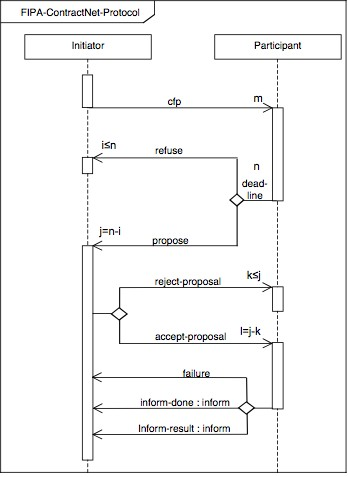
\includegraphics[width=0.4\textwidth]{fipa_cn.png}
\caption{FIPA Contract Net Protocol} \label{f1}
\end{figure}

CNP è stato pensato per assegnare un singolo task all'interno di un gruppo di agenti; tuttavia, in presenza di molteplici \emph{Initiator} e nel caso in cui gli agenti di un MAS abbiano risorse limitate diventa un problema decidere come e in quale istante i \emph{Responder} debbano allocare, e quindi impegnare definitivamente, quelle disponibili. In un simile scenario è del tutto plausibile immaginare che un \emph{Responder} possa ricevere nuove \emph{call for proposal} mentre ha ancora trattative aperte con molteplici \emph{Initiator} impegnati a valutare tutte le proposte:
\begin{itemize}
\item{se l'agente alloca le sue risorse troppo presto tenderà ad essere spesso non disponibile ad accettare nuovi task, rischiando di sprecare risorse qualora le sue offerte venissero rifiutate;}
\item{se l'agente alloca le sue risorse troppo tardi corre il rischio di accettare più task di quelli per cui ha risorse sufficienti.}
\end{itemize}
Nella sez.\ref{s1} verranno illustrate alcune delle soluzioni esistenti per risolvere i problemi sopra descritti, alle quali ci siamo ispirati per la definizione della nostra proposta, presentata di seguito.

\section{ESTENSIONE DEL CNP} \label{s1}
\subsection*{Approcci esistenti} \label{ss1}
Tra le soluzioni più diffuse e adottate in letteratura ce ne sono alcune che modificano il CNP originale aggiungendo al protocollo ulteriori fasi e scambi di messaggi, con l'obiettivo di definire più chiaramente l'istante in cui gli agenti possono effettivamente allocare le loro risorse ai task da eseguire, e di risolvere le limitazioni sopra descritte. Ci siamo soffermati ad analizzare principalmente la \emph{Iterated Contract Net} (ICN) proposta in \cite{c4}, e la \emph{Holonic Contract Net with Confirmation Protocol} (HCNCP) definita in \cite{c5}.

La soluzione proposta da ICN introduce nuove primitive di conversazione (\emph{performative} dei messaggi): i messaggi \emph{cfp}, \emph{accept-proposal} e \emph{reject-proposal} vengono sostituiti da \emph{PreBid}, \emph{PreAccept}, \emph{PreReject}, \emph{DefinitiveBid}, \emph{DefinitiveAccept} e \emph{DefinitiveReject}. In questo protocollo:
\begin{itemize}
\item{all'annuncio di un nuovo task i partecipanti rispondono con delle offerte temporanee (\emph{PreBid});}
\item{l'iniziatore manda al migliore tra i partecipanti un'accettazione temporanea (\emph{PreAccept}), e a tutti gli altri un rifiuto temporaneo (\emph{PreReject});}
\item{chi ha ricevuto una \emph{PreAccept} può inviare una \emph{DefinitiveBid} per confermare la sua offerta, mentre gli altri possono inviare nuove \emph{PreBid} finché non ricevono una \emph{DefinitiveReject} dall'iniziatore;}
\item{l'iniziatore confronta la \emph{DefinitiveBid} con tutte le nuove \emph{PreBid} ricevute: se c'è una \emph{PreBid} migliore della \emph{DefinitiveBid} verrà inviato un nuovo \emph{PreAccept} al partecipante corrispondente, altrimenti l'iniziatore invierà una \emph{DefinitiveAccept} al vincitore e \emph{DefinitiveReject} a tutti gli altri.}
\end{itemize}
Una rappresentazione della sequenza di passi di questo protocollo è riportata in fig.\ref{f2}.

\begin{figure}[!b]
\centering
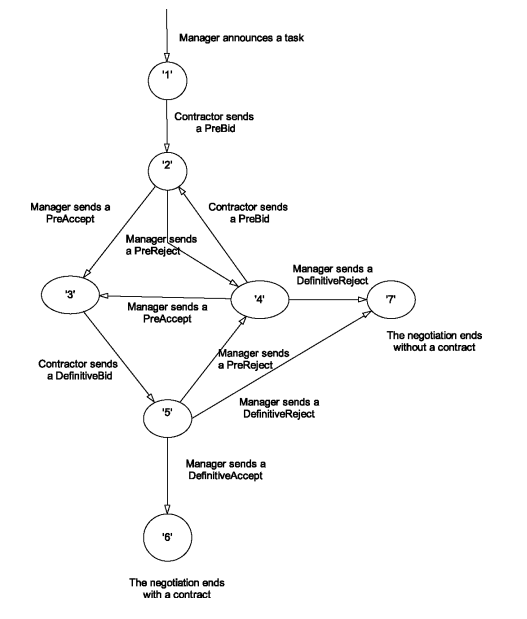
\includegraphics[width=0.4\textwidth]{icn.png}
\caption{Grafo delle transizioni di stato del protocollo Iterated Contract Net} \label{f2}
\end{figure}

Il problema principale che riscontriamo in questo modello di interazione è che non è specificato nel protocollo un numero massimo di volte per cui i partecipanti che ricevono una \emph{PreReject} possono inviare un nuovo \emph{PreBid}: l'iniziatore deve continuamente rivalutare le nuove \emph{PreBid} che arrivano dagli $n - 1$ partecipanti che avevano ricevuto una \emph{PreReject}, e potrebbe rimanere bloccato in questa fase per un tempo indefinitamente lungo se la \emph{DefinitiveBid} non è mai migliore delle nuove \emph{PreBid} ricevute, specialmente per $n$ (numero di partecipanti) grande. Inoltre l'introduzione di nuove performative al di fuori di quelle FIPA potrebbe rappresentare un problema per l'implementazione di una versione \emph{standard-compliant}.

Per quanto riguarda HCNCP invece:
\begin{itemize}
\item{l'iniziatore mantiene in una lista ordinata tutte le proposte ricevute e manda una \emph{request} al mittente della prima;}
\item{se il partecipante scelto invia una \emph{refuse} o non risponde entro una deadline viene contattato il partecipante successivo in lista; il processo si ripete finché un partecipante invia una \emph{agree};}
\item{il partecipante che riceve una \emph{request} ha la possibilità, oltre che di accettare o confermare la sua proposta, di ritrattare con un nuovo messaggio \emph{propose} le eventuali condizioni che aveva precedentemente espresso: in questo caso l'iniziatore dovrà decidere se accettare o meno questa nuova offerta.}
\end{itemize}
Un'illustrazione più dettagliata delle fasi del protocollo è riportata in fig.\ref{f3}.

\begin{figure}[t]
\centering
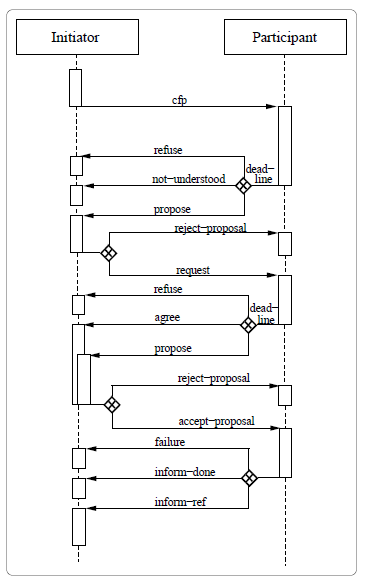
\includegraphics[width=0.4\textwidth]{hcncp.png}
\caption{Holonic Contract Net with Confirmation Protocol} \label{f3}
\end{figure}

La nostra soluzione prende spunto proprio da HCNCP, con qualche modifica che verrà di seguito illustrata.

\subsection*{La nostra soluzione} \label{ss2}
Come già accennato, la nostra proposta di protocollo è una variante del HCNCP già descritto, del quale siamo andati a modificare alcuni dettagli che ci sembrava potessero essere migliorati. Nello specifico:
\begin{itemize}
\item{l'iniziatore non invia più \emph{reject-proposal} in alternativa alla \emph{request}, ma ritarda tale notifica fino al momento in cui accetta (\emph{accept-proposal}) la proposta definitiva (\emph{agree}) del vincitore: dato che al partecipante viene lasciata l'opportunità di fare una seconda proposta, in caso l'iniziatore decida di rifiutarla risulta quindi conveniente tenere in considerazione anche tutte le proposte precedentemente ignorate, in modo da non rimanere con una proposta eventualmente peggiore delle precedenti;}
\item{i partecipanti non inviano più \emph{refuse} in alternativa a \emph{agree} e \emph{propose} per sfruttare maggiormente la possibilità di poter inviare una controproposta, eventualmente con un nuovo costo più conveniente.}
\end{itemize}
Il diagramma delle interazioni del nostro protocollo che rispecchia le modifiche appena illustrate è riportato in fig.\ref{f4}.

\begin{figure}[t]
\centering
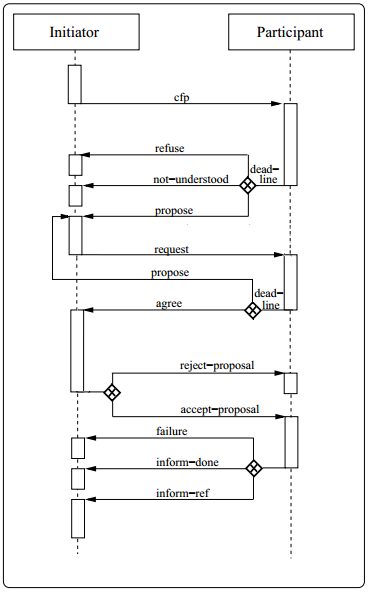
\includegraphics[width=0.4\textwidth]{proto2.png}
\caption{Versione modificata di Holonic Contract Net with Confirmation Protocol} \label{f4}
\end{figure}

Nella prossima sezione verrà presentata l'implementazione di quanto appena descritto in un piccolo programma di esempio, usando il framework per l'\emph{Agent Oriented Programming} JADE.

\addtolength{\textheight}{-9.9cm} % This command serves to balance the column lengths on the last page of the document manually. It shortens the textheight of the last page by a suitable amount. This command does not take effect until the next page so it should come on the page before the last. Make sure that you do not shorten the textheight too much.

\section{IMPLEMENTAZIONE} \label{s2}
Per la nostra demo abbiamo innanzitutto creato due classi, all'interno del package \texttt{agents}, per i nostri due tipi di agenti (corrispondenti ai ruoli \emph{Initiator} e \emph{Responder} definiti dal protocollo). Tali classi estendono la classe \texttt{jade.core.Agent}.
Il passo successivo è stato l'implementazione dei \emph{behaviours}, ovvero dei comportamenti specifici di ciascun ruolo: in particolare abbiamo creato, in un package \texttt{behav}, le classi:
\begin{itemize}
\item{\texttt{SubInit}: è uno dei behaviour appartenenti agli agenti iniziatori; estende la classe \texttt{jade.proto.SubscriptionInitiator}. Si occupa della fase di \emph{discovery} degli agenti che potrebbero essere in grado di completare determinati task, che non è definita formalmente né da CNP né dalle sue estensioni menzionate in questa relazione. Nello specifico il behaviour si occupa di inviare al \emph{Directory Facilitator} del \emph{Main-Container} della nostra piattaforma ad agenti un messaggio di richiesta dell'elenco di tutti gli agenti Responder registrati che forniscono il servizio richiesto dall'iniziatore. Tale elenco viene passato a un secondo behaviour (\texttt{ProtoInitiator}), che viene subito schedulato dall'agente.}
\item{\texttt{ProtoInitiator}: è un altro behaviour degli agenti iniziatori; estende la classe \texttt{jade.core.behaviours.FSMBehaviour}. Equivale alla definizione del protocollo per il ruolo \emph{Initiator}, le cui fasi vengono gestite tramite una macchina a stati. Tali stati e le relative transizioni sono state definite da noi in conformità con la definizione del nostro protocollo.}
\item{\texttt{ProtoResponder}: è un behaviour degli agenti \emph{Responder} (i partecipanti); estende la classe \texttt{jade.core.behaviours.ParallelBehaviour}. Permette agli agenti di poter partecipare a più trattative (sessioni del protocollo) contemporaneamente gestendo le risorse disponibili tra tutte; è composto da un sub-behaviour di tipo \texttt{CyclicBehaviour} che, schedulato dall'agente con criterio \emph{round-robin}, rimane in attesa di ricevere eventuali nuove \emph{call for proposal} e rispondendo con la creazione di una nuova istanza del ruolo \emph{Responder} (\texttt{SSProtoResponder}) del nostro protocollo.}
\item{\texttt{SSProtoResponder}: estende la classe \texttt{jade.core.behaviours.FSMBehaviour}: in maniera corrispondente a \texttt{ProtoInitiator}, definisce una macchina a stati equivalente alla definizione e al funzionamento del nostro protocollo per il ruolo \emph{Responder}.}
\end{itemize}
Per mostrare il funzionamento del protocollo da noi definito, abbiamo creato un piccolo programma che crea alcuni agenti \emph{Initiator} e altri \emph{Responder}, con valori (numerici) di risorse e costi generati casualmente (con la possibilità di specificarli direttamente come parametri degli agenti del programma tramite linea di comando), dove ciascuno degli iniziatori chiede a tutti i partecipanti di effettuare un task (una semplice stampa a schermo). Usando lo strumento \emph{Sniffer} della GUI di JADE si può visualizzare la sequenza di messaggi scambiati tra i diversi agenti come previsto dal nostro modello di interazione. La fig.\ref{f5} riporta lo screenshot di un'esecuzione in cui erano presenti due \emph{Initiator} e due \emph{Responder}.

\begin{figure}[t]
\centering
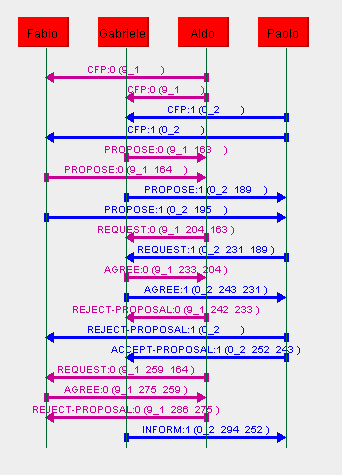
\includegraphics[width=0.4\textwidth]{sniffer.png}
\caption{Schermata di un'esecuzione del programma} \label{f5}
\end{figure}

\section{CONCLUSIONI} \label{s3}
Nella prima parte di questo articolo abbiamo presentato il protocollo Contract Net nella sua versione originale, e nelle sue due estensioni più famose in letteratura. Abbiamo quindi definito una variante di una delle due, proponendo accorgimenti migliorativi nella specifica delle diverse fasi. \`{E} da notare il fatto che, invece di impegnarsi nella fase di offerta, gli agenti partecipanti allocano le risorse solo al momento di invio del messaggio di \emph{accept-proposal}. Anche se questo approccio, rispetto al CNP, ha un maggiore overhead per ricercare ripetutamente l'offerta migliore, richiede che un agente si impegni una sola volta, durante la fase di conferma del protocollo. In questo modo un partecipante può rispondere a tutte le \emph{cfp} dei diversi iniziatori senza necessità di allocare risorse prima di ricevere effettivamente il task. Inoltre, il vantaggio di un modello del genere è che può trovare soluzioni al problema dell'assegnamento dei task in sistemi multi-agente con una struttura di delega, che farebbe fallire CNP.

Riguardo alla nostra implementazione, i ruoli di Partecipante e Iniziatore risultano statici, cioè non variano durante una singola interazione. Tuttavia nessuno vieta ad un agente di poter ricoprire entrambi i ruoli, purché in due conversazioni diverse.

In conclusione, possiamo dire di aver presentato una soluzione semplice ed efficiente alle problematiche esistenti del protocollo Contract Net.

\begin{thebibliography}{5}
\bibitem{c1}\emph{FIPA Contract Net Interaction Protocol Specification}, \url{http://www.fipa.org/specs/fipa00029/SC00029H.html}.
\bibitem{c2}\emph{Jade Site | Java Agent DEvelopment Framework}, \url{http://jade.tilab.com/}.
\bibitem{c3}R. G. Smith, \emph{The contract net protocol: High level communication and control in a distributed problem solver}, IEEE Transactions on Computers, Series C-29 (1980) 1104-1113.
\bibitem{c4}S. Aknine, S. Pinson, M. F. Shakun, \emph{An extended multi-agent negotiation protocol}, Autonomous Agents and Multi-Agent Systems 8 (2004) 5–45.
\bibitem{c5}T. Knabe, M. Schillo, K. Fischer, \emph{Improvements to the fipa contract net protocol for performance increase and cascading applications} (2002).
\end{thebibliography}
\end{document}
